% !TEX root = ../../prj4projektrapport.tex
% SKAL STÅ I TOPPEN AF ALLE FILER FOR AT MASTER-filen KOMPILERES 

\section{Test}

I dette afsnit vil der ikke blive gået i dybden med de enkelte tests, men derimod selve testprocessen og tankerne gjort i testfasen. For at se mere om de enkelte udførte test, se dokumentationen\footnote{Projektdokumentation, 10.4, Modultest}.

Da Styringsenheden generelt har indeholdt meget programmering, har det været oplagt at teste funktionaliteten af koden på nogle enheder på andre allerede udviklede og testede moduler i projektet.  Eksempelvis er funktionaliteten af Brugergrænsefladen testet med brug af andre allerede testede moduler. Til testen af Brugergrænsefladen er kommunikationen fra Måleenhed til Kommunikationsmodul og videre til Kontrolmodulet brugt for at genere tilfældige data, der så blev sendt til og udskrevet på HMI'en fra Kontrolmodulet. Det samme gælder testen af Arduinoens TCP modtagefunktion. Her er PLC'en benyttet  med et testprogram, der kan sende 'req1' kommandoen. Da man allerede har testet PLC'ens forbindelse på et andet Winsock testprogram, kan testen fokusere på Arduinoen. Herunder ses et enkelt testeksempel, hvor dette test program har været benyttet, se figur \ref{fig:EthernetTest}. For hele testbeskrivelsen refereres til dokumentationen\footnote{Projektdokumentation, 10.4.1, Kontrolmodul}.


\begin{figure}[H] % (alternativt [H])
	\centering
	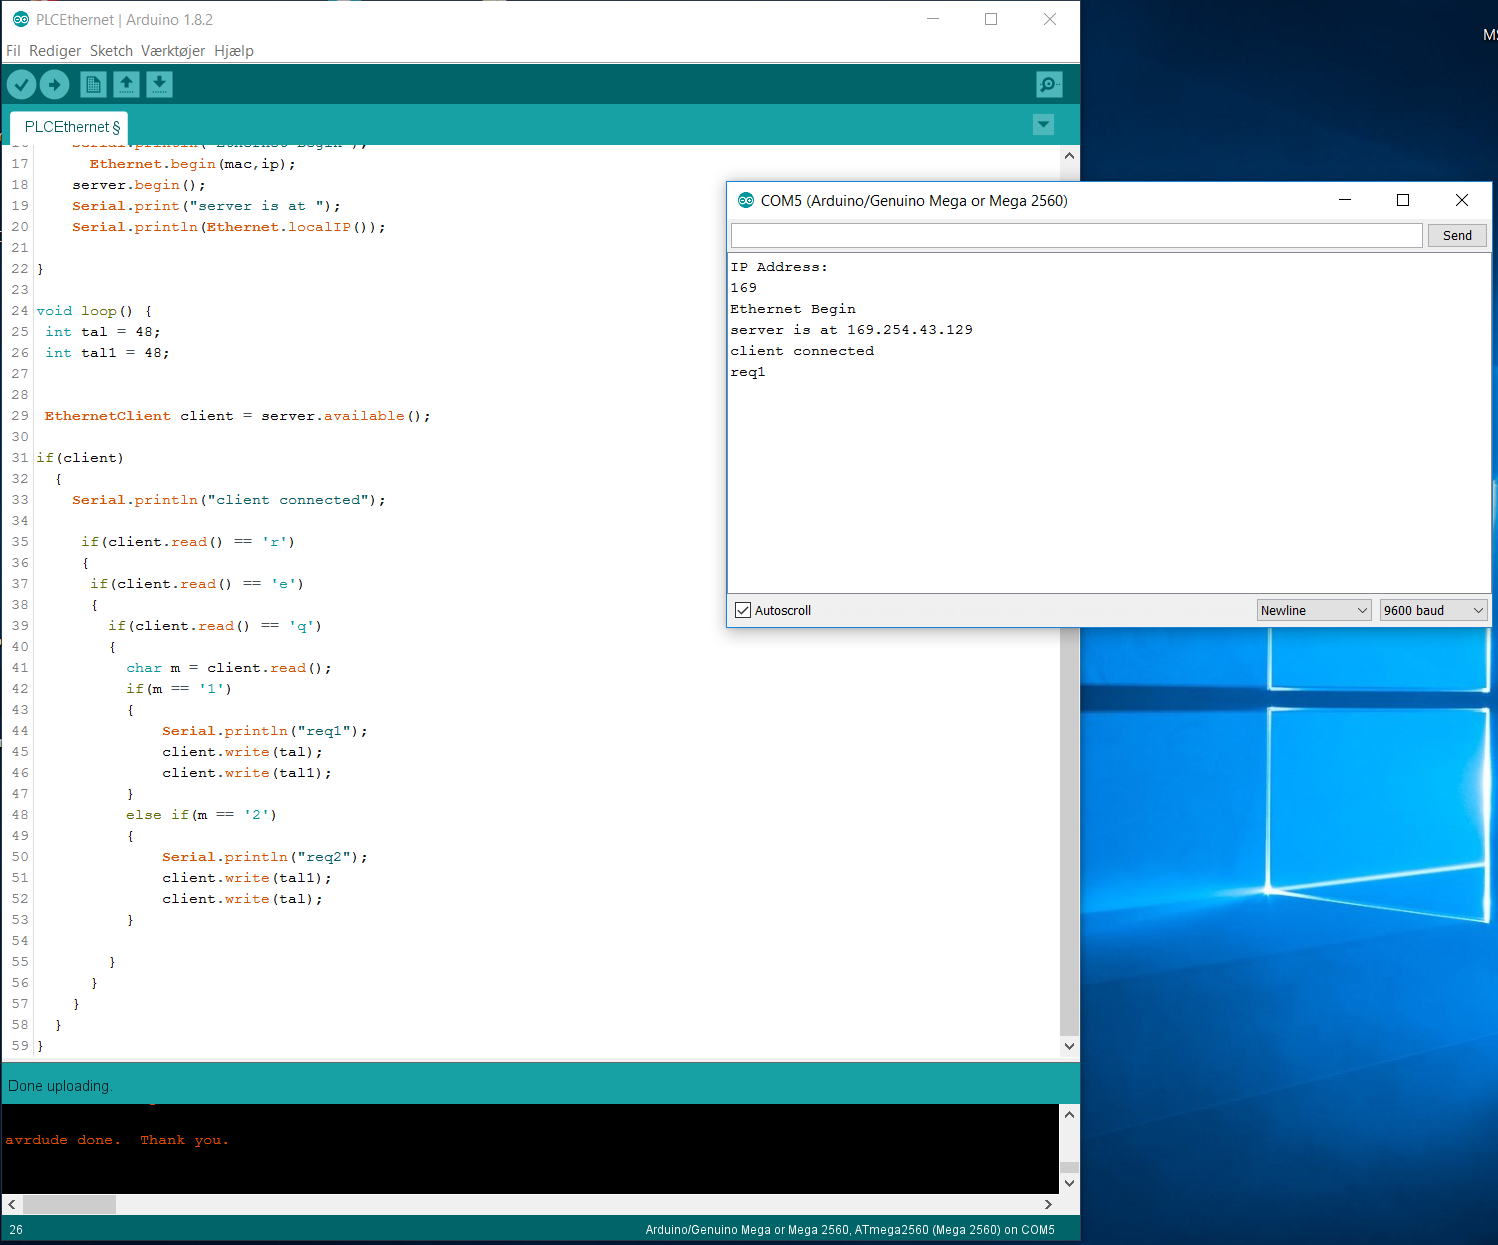
\includegraphics[width=0.85\textwidth]{figure/EthernetTest}
	\caption{Test af Arduinoens TCP data modtagelse}
	\label{fig:EthernetTest}
\end{figure}

